\chapter{Grundlagen}
\label{sec:grundlagen}
In diesem Kapitel werden die Grundlagen, die eine Evalution der Grid Fins ermöglicht, vorgestellt. Um in nächsten Kapitel eine bestmögliche Finne zu entwerfen, sind diese Kenntnisse über die Steuerelemente an sich und den Missionsverlauf unabdingbar.
Zuerst werden nun also Grid Fins, wie sie beschrieben werden können und was für Eigenschaften sie besitzen, vorgestellt. Dabei werden sie mit planaren Finnen verglichen und anschließend wird auf bisherige Implementationen eingegangen. Zuletzt wird noch auf das AirLaunch-System Valkyrie eingegangen.
\section{Aufbau von Grid Fins}
Um Grid Fins und ihre Orientierung beschreiben zu können, werden zunächst einige Größe eingeführt.
In der simpelsten Konfiguration bestehen Grid Fins aus einem äußeren Rahmen, der die innere Struktur von sich kreuzenden planaren Flächen stützt. Dieser einfache Aufbau gewährt hohe Stabilität bei vergleichsweise geringem Gewicht \cite{zellform}.
\subsection{Parameter}
Diese Struktur lässt sich mittels 5 Parameter, wie in Abbildung \ref{abb_parameter} zu sehen, beschreiben. Die Wanddicke $\gls{symb:d}$ kann sich für den Rahmen ($d_{\gls{Index:R}}$) von der des Gitters ($d_{\gls{Index:G}}$) unterscheiden. Aber auch innerhalb dieser Einteilung kann der Wert variieren. So ist häufig die Wandstärke in der Nähe der Einspannung erhöht, um die dort auftretenden höheren Beanspruchungen zu ertragen. Ein von den Wänden umrahmter Durchlass des Gitters wird als Zelle bezeichnet und seine Abmessung kann mit die Zellgröße $\gls{symb:g}$ beschrieben werden. Die Ausmaße der Grid Fins werden maßgeblich durch die Spannweite $\gls{symb:b}$ und die Höhe $\gls{symb:h}$ bestimmt. Die Querschnittsfläche $\gls{symb:A}$ steht in der Ausgangsstellung senkrecht zur Anströmung und wird vom Rahmen begrenzt. Normal zu dieser Fläche steht die Sehne mit einer im Vergleich zur planaren Finne deutlich kürzeren Länge $\gls{symb:s}$.\\
\begin{figure}[h]
	\centering
	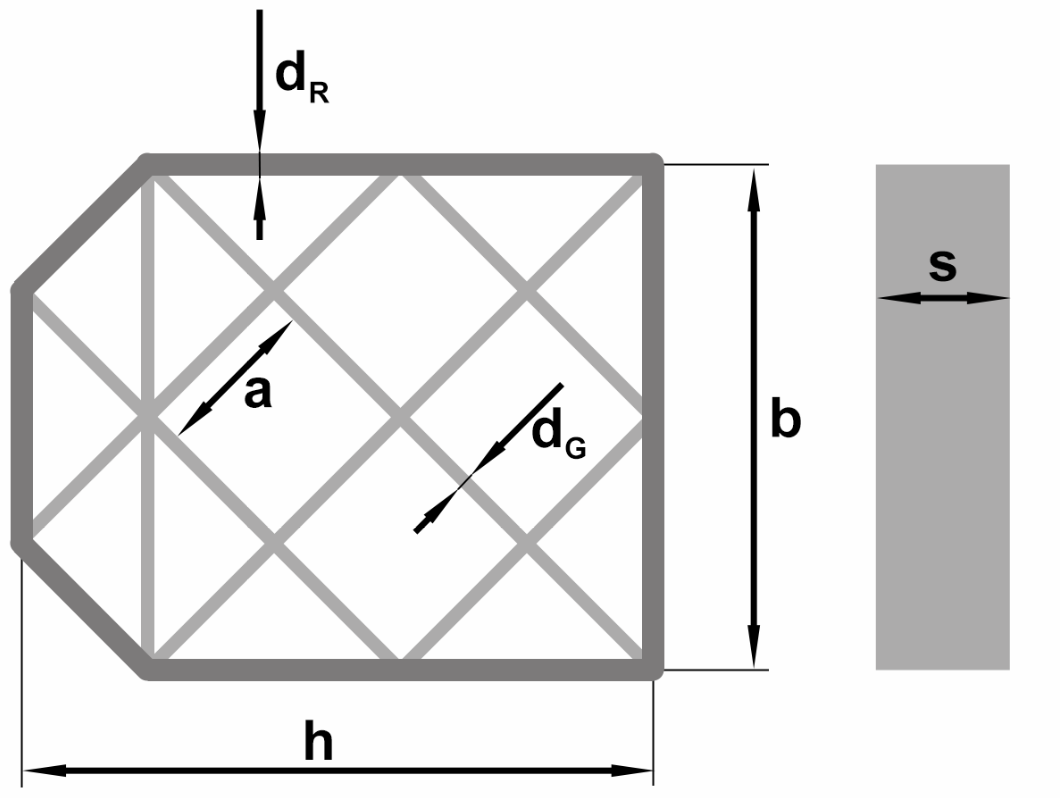
\includegraphics[width=0.6\textwidth]{Parameter.png}
	\caption{Aufbau eines einfachen Grid Fins}
	\label{abb_parameter}
\end{figure}\\
\subsection{Orientierung}
Grid Fins müssen nicht starr an einem Flugkörper, zum Beispiel der Rakete, befestigt werden, sondern können um mehrere Achsen drehbar sein. Abbildung \ref{abb_winkel} zeigt die wichtigsten Winkel aus jeweils verschiedenen Ansichten an einem Flugkörper. Um Grid Fins für den Transport kompakt zu lagern, lassen sie sich an den Körper anlegen. Der Klappwinkel $\gls{symb:Lambda}$ beschreibt den Ausschlag um eine den Körper an der Anbringung tangierende Achse. Ein Klappwinkel von $0^\circ$ entspricht hierbei dem normalen in die Strömung ragenden Zustand und $90^\circ$ dem eingeklappten. Zur Steuerung lassen sich die Grid Fins um eine Achse, die orthogonal aus dem Körperoberfläche durch die Mitte des Grid Fins zeigt, verstellen. Ein Steuerwinkel von $\eta = 0^\circ$ ist auch hier wieder die Ausgangsstellung, die Sehne ist parallel zur X-Achse. Bei $\eta = 90^\circ$ würde also die Seitenkante zur Anströmung zeigen. Die Querschnittsfläche $A$ und somit also auch das Gitter wird nicht durchströmt.
\begin{figure}[h]
	\centering
	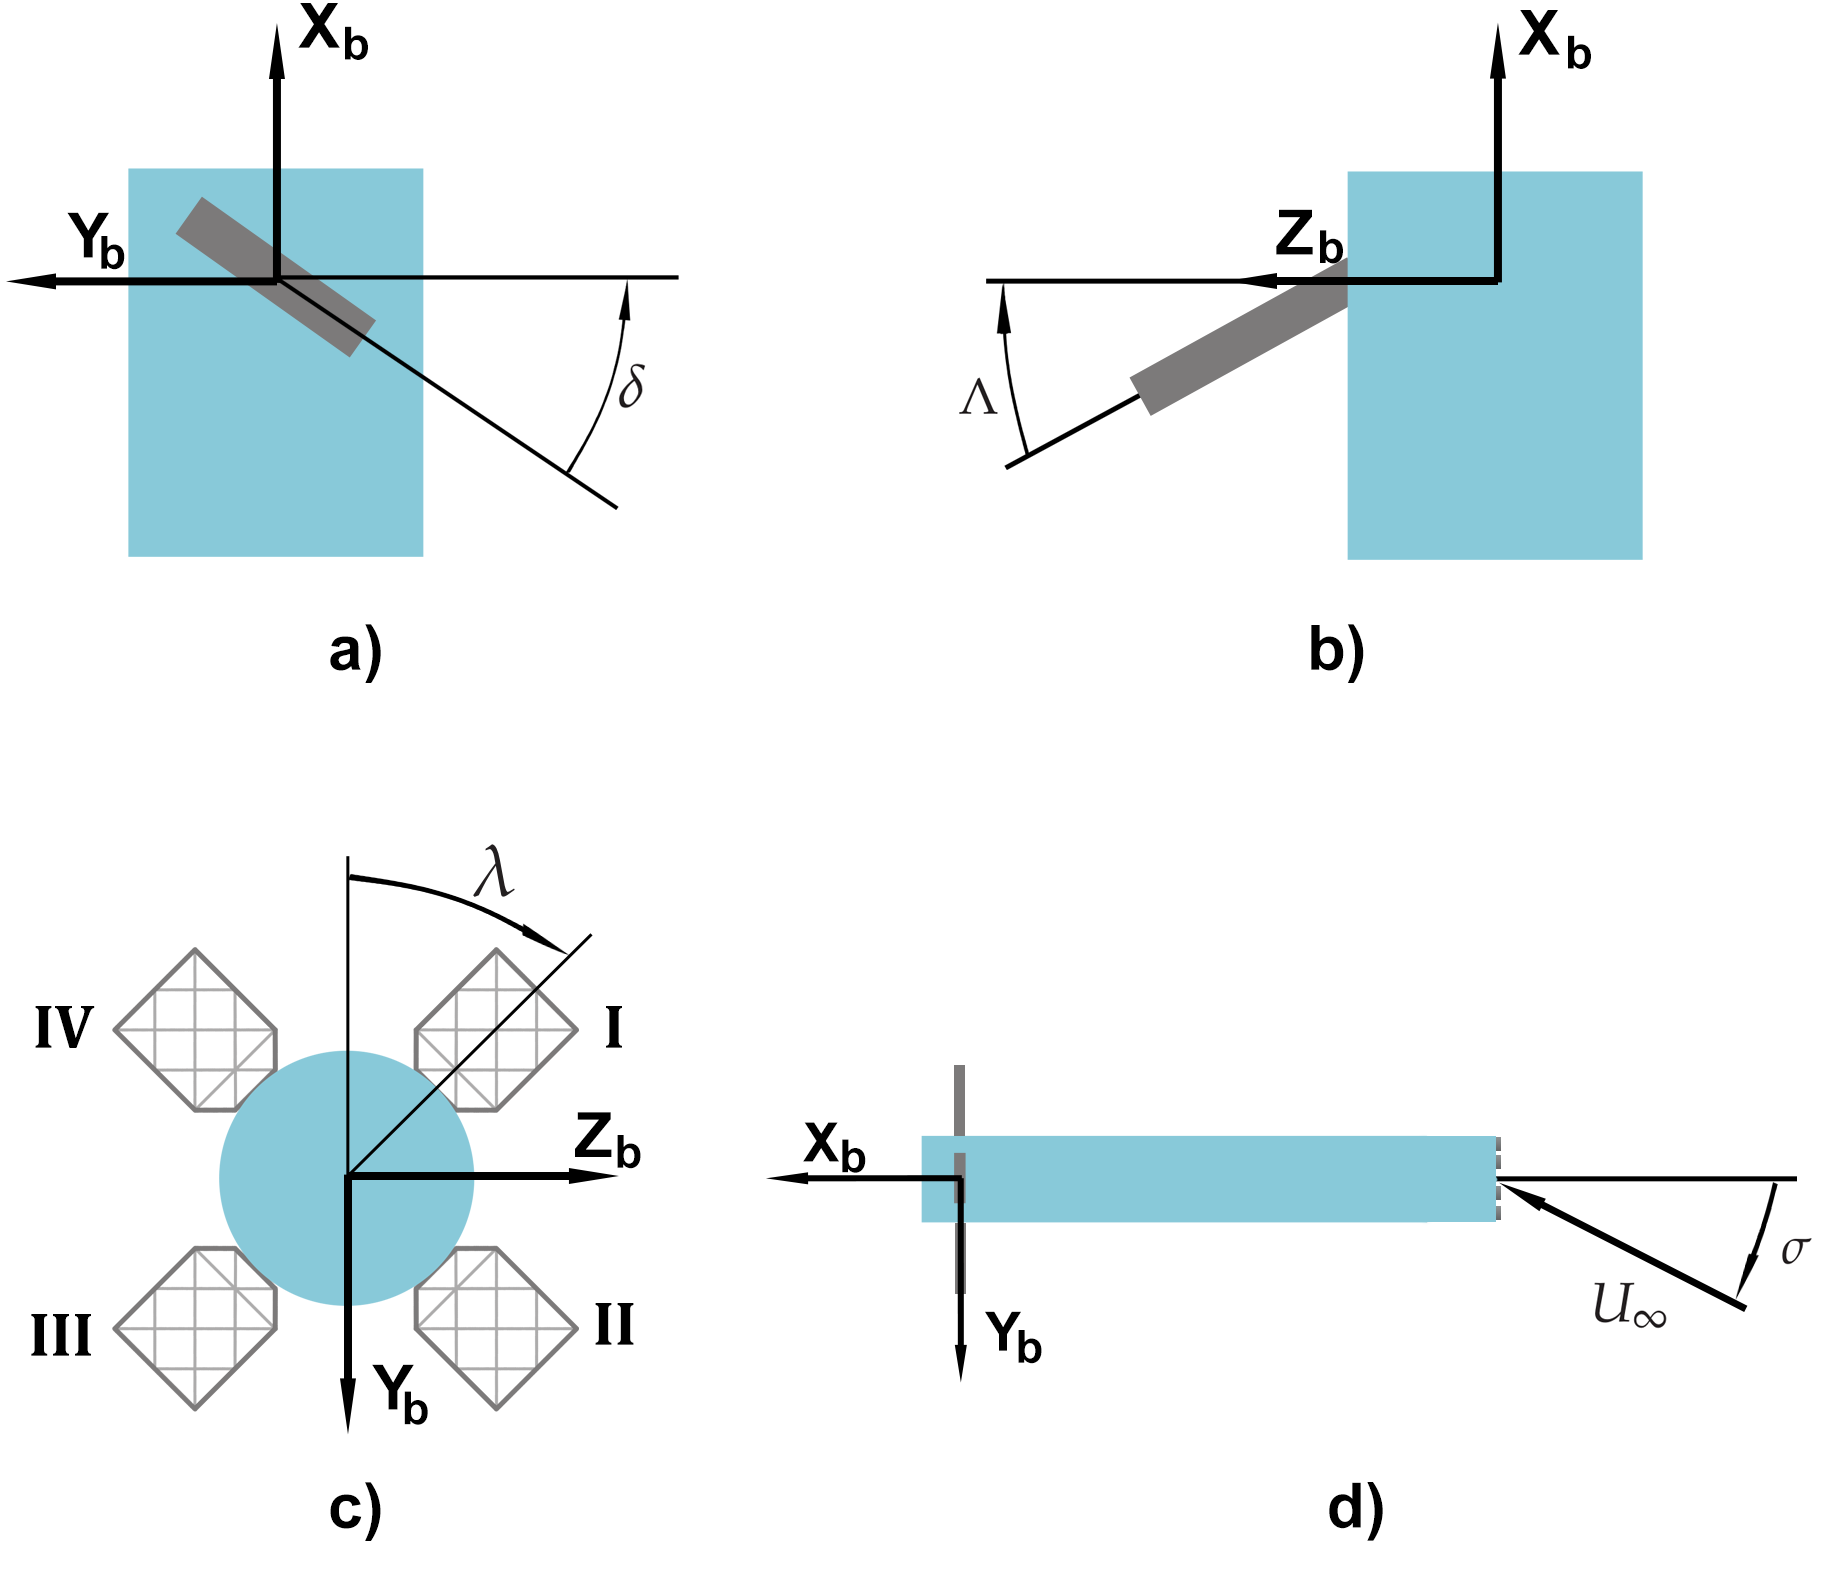
\includegraphics[width=0.8\textwidth]{Winkel.png}
	\caption{Winkel zur Beschreibung der Orientierung der Grid Fins zum Körper\\a) Steuerwinkel, b) Klappwinkel, c) Drehwinkel, d) Neigungswinkel des Körpers zur Anströmung}
	\label{abb_winkel}
\end{figure}\\
Um die Aerodynamik zu untersuchen reichen diese Winkel nicht aus, da die Anströmung nicht parallel zur Rakete liegen muss. Der Neigungswinkel des gesamten Moduls zur Anströmung $\gls{symb:sigma}$ setzt sich unter realen Bedingungen mit Vernachlässigung des Windes aus dem Schiebewinkel und dem Bahnneigungswinkel zusammen. Für die in dieser Arbeit durchgeführten Untersuchungen ist eine solche Aufteilung aber irrelevant. Damit aber keine Informationen und somit Genauigkeit verloren geht, wird stattdessen die Orientierung der Grid Fins auf dem Umfang betrachtet. Verwendet wird hier eine Anordnung von vier gleichmäßig verteilten Steuerelementen. Das Koordinatensystem ist so definiert, dass es seinen Ursprung genau in der Mitte dieser Konfiguration hat und die positive X-Achse zur Spitze des Flugkörpers, also entgegen der Anströmung, zeigt. Bei $\sigma \neq 0$ zeigt auch die Y-Achse einem Anteil der Strömung entgegen. Die Z-Achse ist folglich nach dem Rechtssystem orthogonal zu den anderen beiden ausgerichtet. Um nun die Orientierung der Grid Fins um die X-Achse herum beschreiben zu können wird der Rollwinkel $\gls{symb:lambda}$ eingeführt. Wenn eine '+'-Konfiguration vorliegt, befinden sich die einzelnen Finnen auf den Koordinatenachsen (X, Y) und der Rollwinkel ist gleich null. Im Gegensatz dazu sind sie bei der 'x'-Konfiguration um einen Winkel von $\lambda = 45^\circ$ verdreht. Der Anstellwinkel $\gls{symb:alpha}$, den ein einzelner Grid Fin erfährt, lässt sich aus dem Neigungswinkel des Körpers und, in Abhängigkeit vom Rollwinkel und welcher der Finnen betrachtet wird, aus dem Klapp- und Steuerwinkel bestimmen.
\newpage

\section{Strömung durch Grid Fins}\label{stroe}
Um die Eigenschaften von Grid Fins analysieren zu können, ist es nötig die zugrunde liegenden strömungsmechanische Vorgänge zu verstehen. Dazu wird in diesem Abschnitt das Verhalten der Strömung im Unter-, Überschall und besonders auch im transsonischen Bereich mit Schwerpunkt auf die dort wirkenden Verdichtungsstöße besprochen.
Bei niedrigen Strömungsgeschwindigkeiten im Unterschall haben Grid Fins auf Grund ihrer geringen Dicke keinen großen Einfluss auf das Fluid, welches nahezu ungestört durch das Gitter fließen kann \cite{sb-sharp}. Mit steigenden Machzahlen macht sich jedoch zunehmend der Effekt einer um die stumpfe Vorderkante des Gitters herum in die Zelle hinein expandierende Strömung bemerkbar. Zusammen mit der Grenzschichtbildung an den Zellwänden, die effektiv zu Verengung der durchströmten Fläche führt, wir die Strömung innerhalb der Zellen auf Geschwindigkeiten beschleunigt, die über der Anströmung liegen \cite{synopsis}.
\\~\\
Der transsonische Bereich wird ab einer Anströmungsmachzahl von circa $Ma_\infty=0,8$ erreicht \cite{machgrenzen} und stellt für die Aerodynamik der Grid Fins eine bedeutsame Problematik dar. Sobald die Strömung innerhalb des Gitters eine Machzahl von $1$ überschreitet, kommt es zu einem Verdichtungsstoß am Ausgang der Zellen, der mit steigender Machzahl an Stärke zunimmt. Dieser führt zu einer Drosselung der Strömung, was zur Folge hat, dass ein Teil der Strömung verdrängt wird und sich stattdessen um den Grid Fin herum bewegt. Steigt nun auch $Ma_{\gls{Index:inf}}$ über $1$ löst sich der Stoß von den Gitterwänden und verbindet sich zu einer unregelmäßigen 3D-Struktur im Nachlauf \cite{stroemung}. Wächst $Ma_\infty$ weiter an, so kommt es zu einem Verdichtungsstoß vor dem Grid Fin. Dies führt dazu, dass innerhalb der Zellen keine Drosselung mehr vorliegt \cite{stroemung}, stattdessen wird die Strömung schon durch den Stoß vor dem Gitter um dieses herum verdrängt \cite{synopsis}. Von den Vorderkanten gehen Schockwellen aus, die auf benachbarte Wände treffen und von ihnen reflektiert werden \cite{synopsis}. Steigt die Machzahl weiter an, so befinden sich diese Wellen auf steileren Bahnen bis sie gar nicht mehr auf die anderen Wände treffen. Abbildung \ref{abb_stoesse} zeigt die Stöße im Unter- (a) und Überschall (b). Auch dargestellt sind die Schockwellen, die entweder von den Wänden reflektiert werden (c) oder unreflektiert hindurch wandern (d).
Des Weiteren nähert sich der Verdichtungsstoß vor dem Grid Fin diesem mit größer werdenden Strömungsgeschwindigkeiten immer weiter an, bis es abgesehen von der direkten Umgebung der Wände zu keinem Stoß mehr kommt. Die einzelnen Zellen fungieren nun als Überschalldüse \cite{stroemung}, sodass die Strömung in den meisten Bereichen nicht mehr auf den Unterschall abgebremst wird. Der Stoß wurde vom Gitter "verschluckt".
\begin{figure}[h]
	\centering
	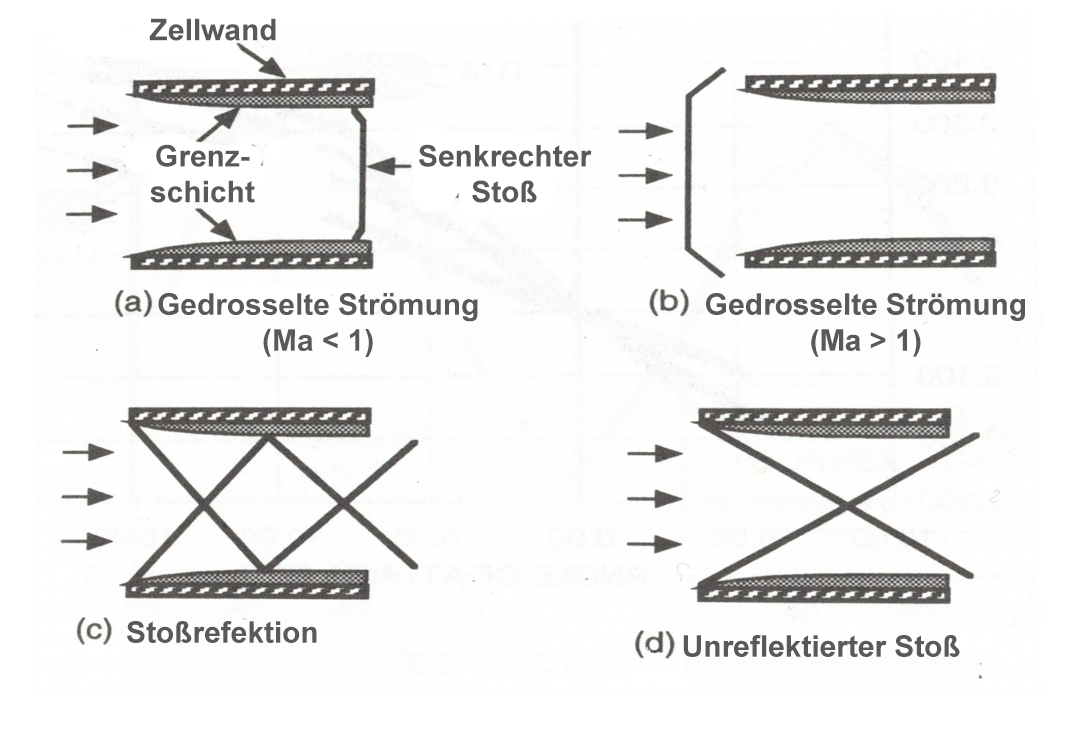
\includegraphics[width=0.7\textwidth]{swallow.png}
	\flushbottom{\cite{synopsis}}
	\caption{Stoßsystem einer Zelle}
	\label{abb_stoesse}
\end{figure}\\
Als ein besonderer Bereich ist noch die Ansatzregion zu betrachten, in der der Grid Fin an der Rakete angebracht ist. Ein Problem ist, dass Schnittstellen von Wänden ein erhöhtes Potenzial für blockierte Strömung darstellen. In der Ansatzregion befinden sich nicht nur vielen von diesen, sondern auch die Wanddicke ist hier meistens am größten. Dies in Kombination mit einer schon durch die Grenzschichtwirkung des Körpers verzögerte Strömung, führt zu einer relativ großen Region verlangsamter Strömung oder gar Rückströmung, die mit der Machzahl an Größe gewinnt \cite{stroemung}. Bei einer Machzahl von ungefähr $Ma_\infty = 2$ erreicht sie jedoch ein Maximum, da die Strömung bei weiter steigenden Geschwindigkeiten von der umgebenden mitgerissen wird und jene Region somit wieder an Größe und Bedeutung verliert \cite{stroemung}.

Es ist nun also hervorzuheben, dass Grid Fins weder im Unterschall noch im hohen Überschall übermäßig starke Störungen der Strömung bewirken. Im transsonischen Bereich jedoch kommt es zu massiven Verdichtungsstößen, die zu einer starken Drosselung des Fluids führen.
\newpage

\section{Aerodynamische Beiwerte und Vergleich zu planaren Finnen}
Nachdem nun die zugrunde liegende Strömung verstanden ist und Größen zur Beschreibung von Grid Fins etabliert wurden, werden nun die aerodynamischen Kräfte beschrieben und dabei der Vergleich zu den konventionellen planaren Finnen gezogen.

Relevant sind zum einen die Normalkraft, die orthogonal zur X-Achse, also in der X-Y-Ebene, liegen ($\gls{symb:F}_{\gls{Index:N}}$) und zum anderen die Axialkraft, die in negative X-Richtung zeigen $F_{\gls{Index:X}}$. In der Ausgangsstellung bei einem Neigungswinkel von $\sigma = 0$ entsprechen sie dem Auftrieb und Widerstand. Zusätzlich ist auch noch das Moment $\gls{symb:M}_{\gls{Index:m}}$ um die Achse in der die Grid Fins steuerbar gelagert ist relevant. Diese Kräfte sind in Abbildung \ref{abb_kraefte} zu erkennen.
\begin{figure}[h]
	\centering
	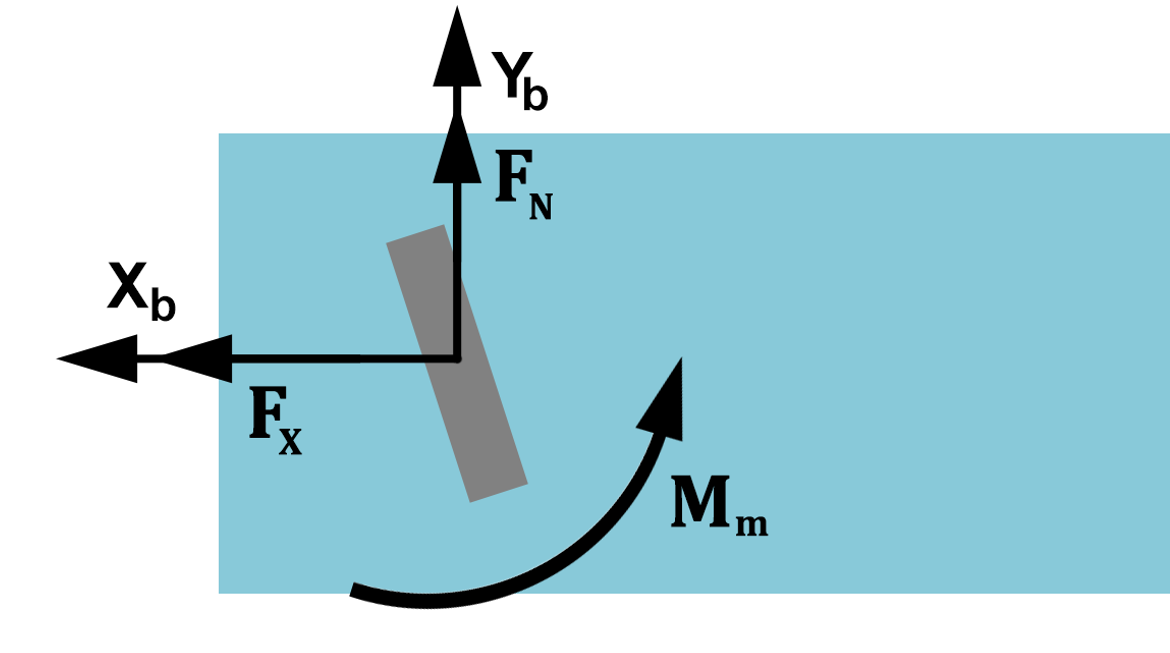
\includegraphics[width=0.6\textwidth]{kraefte.png}
	\caption{Kräfte und Momente am Grid Fin}
	\label{abb_kraefte}
\end{figure}\\
\subsection{Normalkraft}
Die Normalkrafterzeugung ist ausschlaggebend für die Stabilität und Steuerbarkeit eines Flugkörpers. Die Steigung der Normalkraftkoeffizient über den Anstellwinkel $\gls{symb:C}_{N\alpha}$ bei einem Anstellwinkel von $\alpha = 0$ ist in Abbildung \ref{abb_bucket} in Abhängigkeit von der Machzahl zu sehen. Wie in Abschnitt \ref{stroe} beschrieben, führt die Drosselung im transsonischen Bereich dazu, dass die Strömung um den Grid Fin herum verdrängt wird. Dieser Anteil des Fluids kann nicht mehr zur Normalkrafterzeugung beitragen, sodass er einen nicht vernachlässigbaren Teil seiner Fähigkeit diese Kraft zu erzeugen einbüßt. Dieser Effekt ist genau gegensätzlich zu konventionalen planaren Finnen, die im Transschall ihren maximalen Normalkraftkoeffizienten $C_N$ erreichen \cite{synopsis}.
\begin{figure}[h]
	\centering
	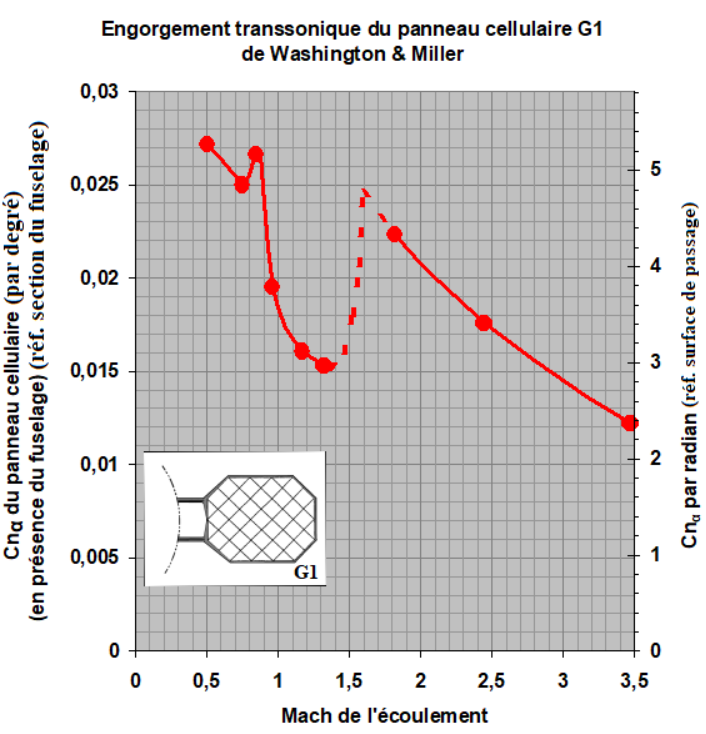
\includegraphics[width=0.6\textwidth]{bucket.png}
	\flushbottom{\cite{synopsis}}
	\caption{Normalkraftsbeiwertgradient bei $\alpha = 0$ in Abhängigkeit von der Machzahl}
	\label{abb_bucket}
\end{figure}\\
Während vergleichbare konventionelle Finnen im Unterschall und niedrigen Überschall ähnlich hohe Normalkräfte erzeugen können, werden sie im hohen Machbereich von Grid Fins übertroffen. Schon ab $Ma=2,5$ kann die Normalkraft das 1,5-fache betragen und dieser Wert steigt mit der Machzahl nur noch weiter an \cite{synopsis,vergleichPlanarNATO}.
\subsection{Axialkraft}
Die Axialkraft wird häufig als der größte Nachteil von Grid Fins angesehen, auch wenn er sich für spezielle Anwendungen sogar als \grqq drag brake\grqq \ nutzen lässt. Wie schon im Abschnitt \ref{stroe} erwähnt, wird die Strömung bei niedrigen Geschwindigkeiten nicht stark gestört, folglich kommt es auch nicht zu großen Axialkräften. Im transsonischen Bereich steigt der Beiwert durch die Drosselung der Verdichtungsstöße rasant an und erreicht bei einer Machzahl knapp unter 1 sein Maximum \cite{solver}. Danach nimmt der Wert wieder ab und bleibt im Überschall nahezu konstant, während er für planare Finnen abnimmt \cite{vergleichPlanarNATO}. Dieser Verlauf des Widerstandsbeiwerts ist auch in Abbildung \ref{abb_Cd-Ma} in Abhängigkeit von der Machzahl für verschiedene Anstellwinkel zu sehen. Generell kann die Axialkraft von Grid Fins das bis zu drei- oder  vierfache des konventionellen betragen.
\subsection{Gelenkmoment}
Ein großer Vorteil von Grid Fins ist ihr geringes Moment um das Steuergelenk, welches den Einsatz von kleineren, weniger leistungsstarken Aktuatoren ermöglicht. Was wiederum eine Einsparung an Gewicht und Kosten mit sich bringt. Der Grund für das niedrige Moment ist hauptsächlich die im Vergleich zur planaren Finne deutlich kürzere Sehne, die der Luftkraft nur einen kleinen Hebelarm bietet. Der Druckpunkt befindet sich schon bei niedrigen Machzahlen in der Nähe der Mitte der Sehne, durch diese Mitte geht gleichzeitig die Achse, um die der Grid Fin gedreht wird, und wandert mit steigender Machzahl wenn auch nur leicht weiter Richtung 50\% der Sehnenlänge \cite{vergleichPlanarNATO}. Dies führt dazu, dass das Gelenkmomentbeiwert $C_m$ mit steigender Machzahl abnimmt. Ebenso wie bei der Axialkraft befindet sich das Maximum bei Machzahlen knapp unter 1, wie in Abbildung \ref{abb_Mm-Ma} zu sehen. Auch für Variationen des Anstellwinkels beleibt der Beiwert durchgehend auf einem niedrigen Niveau, deutlich unter dem seines planaren Gegenstücks \cite{vergleichPlanarNATO}. Es sei hier jedoch anzumerken, dass es möglich ist eine planare Steuerfläche mit einem geringeren Moment zu erhalten, indem die Gelenkachse durch den Druckpunkt gelegt wird. Durch die große Druckpunktwanderung ist dies aber nur für einen kleinen vorher gewählten Machzahlengebiet dem Grid Fin überlegen, der über einen großen Geschwindigkeitsgebiet konstant gute Charakteristiken bietet.
\begin{figure}[h]
	\begin{minipage}[t]{0.45\linewidth}
		\centering
		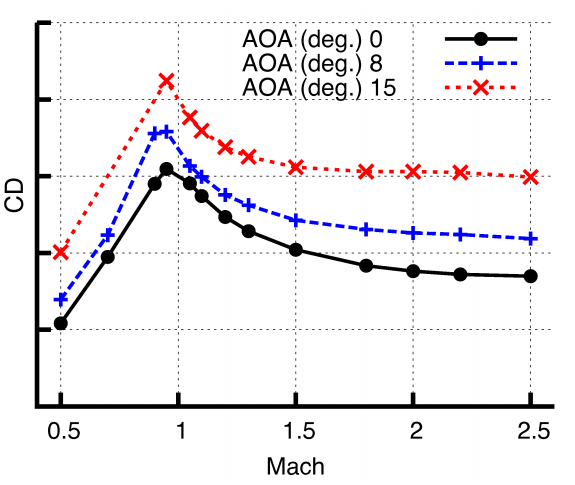
\includegraphics[width=0.85\textwidth]{Cd-Ma.png}
		\flushbottom{\cite{solver}}
		\caption{Axialkraft (hier CD) bei unterschiedlichen Anstellwinkeln in Abhängigkeit von der Machzahl}
		\label{abb_Cd-Ma}
	\end{minipage}
	\hfill
	\begin{minipage}[t]{0.45\linewidth}
		\centering
		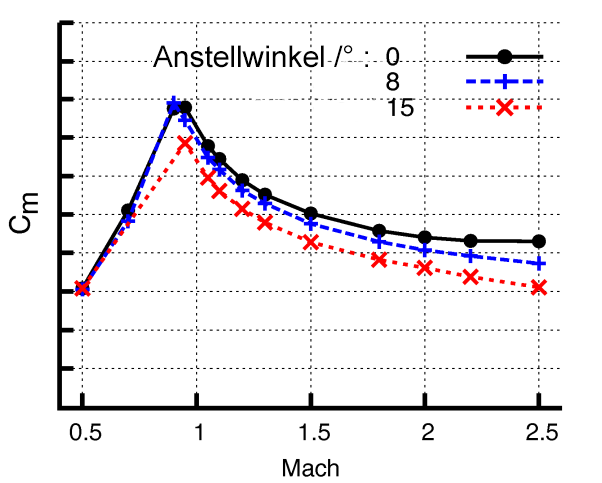
\includegraphics[width=0.9\textwidth]{gelenkmomentMa.png}
		\flushbottom{\cite{solver}}
		\caption{Gelenkmomentenbeiwert bei unterschiedlichen Anstellwinkeln in Abhängigkeit von der Machzahl}
		\label{abb_Mm-Ma}
	\end{minipage}
\end{figure}
\subsection{Stabilität}
Für die statische Stabilität eines Flugkörpers muss bei Neigungswinkeln $\sigma \neq 0$ ein Moment um den \gls{SP} entstehen, das die Orientierung der Körperachse wieder parallel zur Strömung ausrichtet. Grid Fins haben hier einen entscheidenden Vorteil gegenüber planaren Alternativen, da bei ihnen auch die Finnen, die bei einem Rollwinkel von $\lambda = 0$ vertikal ausgerichtet sind, zu diesem Moment beitragen. Selbst der Effekt von Wirbel auf die lee-Finne ist dadurch negiert, dass sich die Variation des lokalen Anstellwinkels über die vergleichsweise große durchströmte Querschnittsfläche ausgleicht. Somit tragen die vertikalen Grid Fins über den gesamten Machbereich mit ungefähr 30\% einen signifikanten Teil zur Stabilität bei \cite{vergleichPlanarNATO}. Das Rückstellmoment um den Schwerpunkt ist sowohl im Unterschall als auch im Überschall größer, nur im Transschall büßen auch hier die Kräfte im Vergleich zur planaren Finne wieder ein.

Die Steuerbarkeit, die Fähigkeit Momente zu generieren, die die Orientierung des Flugkörpers aus der stabilen Lage heraus verändern, ist dadurch jedoch leicht behindert. Wenn zwei gegenüberliegende Grid Fins einen Steuerwinkelausschlag erfahren und somit eine Normalkraft erzeugen, wirken die anderen beiden dieser Kraft mit den soeben angesprochenen 30\% entgegen.
\subsection{Anstellwinkelcharakteristik}
Im Gegensatz zu planaren Finnen, die bei hohen Anstellwinkeln Strömungsabriss erfahren, zeigen Grid Fins ein deutlich besseres Verhalten. Ihre kurze Sehne senkt die Gefahr der Strömungsablösung deutlich und erlaubt somit eine verlässlichere Normalkraftgenerierung, die sich auch noch bei moderaten Anstellwinkeln weiter steigern lässt. Somit liegt im Unterschall die maximale Normalkraft bei $\alpha = 40^\circ$ ohne jegliche Anzeichen von Strömungsabriss \cite{synopsis}.
Des Weiteren ist der Anstieg dieser Kraft mit dem Anstellwinkel im Überschall bis zu Anstellwinkeln von mindestens $\alpha=15^\circ$ beinahe linear \cite{synopsis}, was eine sehr effektive Steuerung ermöglicht.\\
~\\
Abbildung \ref{abb_Cd-AoA} zeigt das Verhalten des Widerstandbeiwerts in Abhängigkeit von dem Anstellwinkel vom Grid Fin und der planaren Finne im Vergleich.
Zu erkennen ist, dass die Widerstandskraft bei den meisten Machzahlen mit wachsendem Anstellwinkel ein ähnliches Verhalten wie die planaren Steuerflächen \cite{vergleichPlanarNATO} zeigt, deren Werte auch stark ansteigen.
		%\cite{Shape} zeigt anderes Verhalten
\begin{figure}[h]
	\centering
	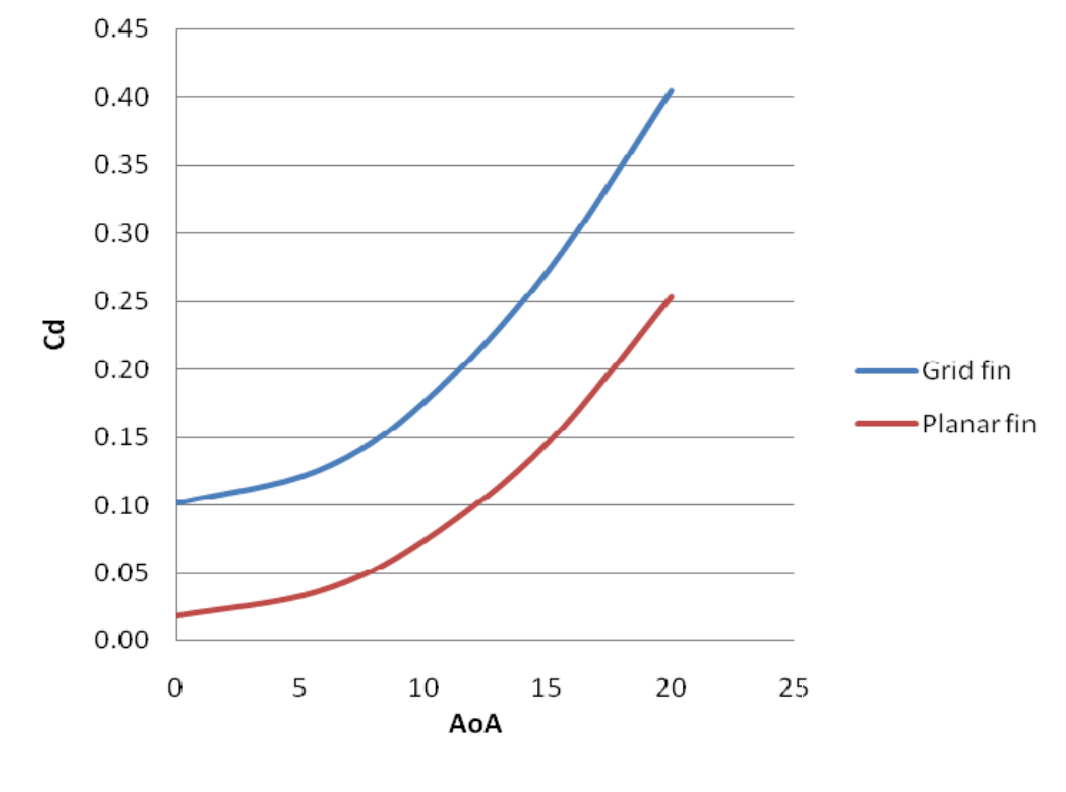
\includegraphics[width=0.5\textwidth]{Cd-AoA.png}
	\flushbottom{\cite{vergleichPlanar}}
	\caption{Widerstandsbeiwert in Abhängigkeit vom Anstellwinkel $\alpha$ bei $Ma=2,5$}
	\label{abb_Cd-AoA}
\end{figure}\\

In Bezug auf das Gelenkmoment $M_m$ zeigen Grid Fins wieder ein überlegendes Verhalten gegenüber planaren Finnen, wie in Abbildung \ref{abb_Mm-AoA} zu sehen ist. Welche dieses in Abhängigkeit vom Anstellwinkel für den Unterschall (a) und Überschall (b) zeigt. Während im Unterschall der Anstieg des Momentes nur geringfügig weniger steil ausfällt und für beide Steuerflächen ab einem Winkel von $\alpha \approx 10^\circ$ beziehungsweise $15^\circ$ zu stagnieren scheint, fällt der Unterschied im Überschall deutlich stärker aus. Die Kurve der planaren Finne zeigt einen rasanten Anstieg bei einer Anströmungsmachzahl von $Ma_\infty = 2,5$, die Steigung des Grid Fins ist jedoch für niedrige Anstellwinkel fast auf demselben Niveau, wie im Unterschall. Erst bei einem Anstellwinkel von circa $\alpha = 15^\circ$ nimmt auch hier die Steigung vergleichbare Werte an. Also ist die Steuerbarkeit bei hohen Machzahlen mit deutlich weniger Leistung möglich. Dies ermöglicht den Einsatz von bedeutend kleineren und somit auch kostengünstigeren Aktuatoren. 
\begin{figure}[h]
	\centering
	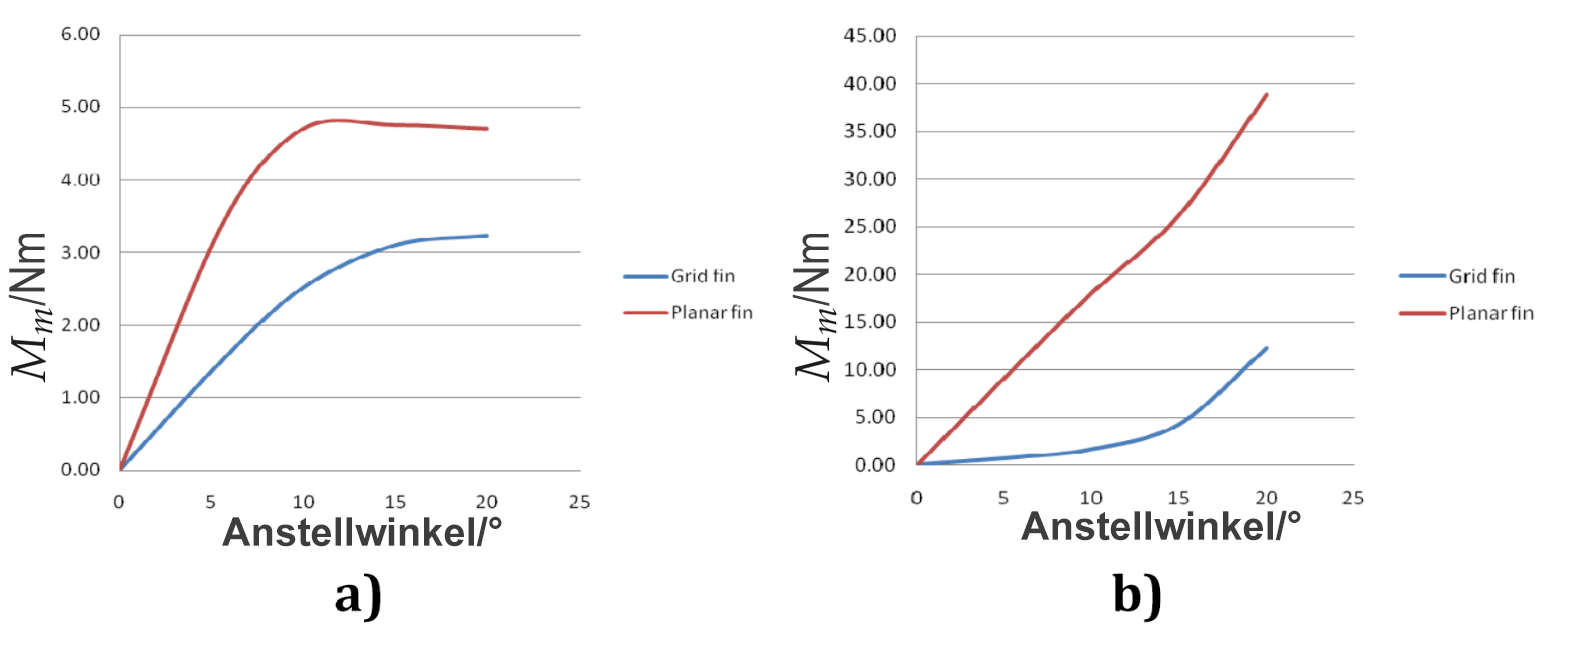
\includegraphics[width=0.8\textwidth]{gelenkmoment.png}
	\flushbottom{\cite{vergleichPlanar}}
	\caption{Gelenkmoment in Abhängigkeit vom Anstellwinkel $\alpha$ bei a) \ensuremath{Ma=0,5}, b) $Ma=2,5$}
	\label{abb_Mm-AoA}
\end{figure}
\newpage
\section{Grid Fin Varianten}
Bisher wurde nur eine sehr simple Version von Grid Fins betrachtet. Es gibt jedoch eine Vielzahl von Variationen, die genutzt werden können, um die aerodynamischen Eigenschaften für bestimmt Anwendungen zu optimieren. In diesem Abschnitt werden einige Möglichkeiten beschrieben, wie diese unkonventionellen Finnen angepasst werden können eingegangen.
\subsection{Pfeilung}
Eine Häufige Kritik von Grid Fins sind ihre hohen Axial- bzw. Widerstandskräfte. Somit ist es nicht verwunderlich, dass ein Großteil der Forschung sich auf die Reduzierung dieses Aspektes konzentriert haben. Eine Häufig gewählte Methode ist hierbei die Pfeilung, deren Nutzen aus den planaren Tragflächentechnik schon seit längerer Zeit bekannt ist. Es wird in dieser Arbeit zwischen drei verschiedenen Varianten unterschieden, wie sich diese Pfeilung auf die komplexe Gitterstruktur übertragen lässt, unterschieden.\\
~\\
Die erste Variante stellt die \textbf{Pfeilung der gesamten Konfiguration} dar. Hierbei beleibt der Grid Fin an sich unverändert. Stattdessen wird die Pfeilung dadurch erreicht, dass die Querschnittfläche nicht senkrecht zur Oberfläche des Flugkörpers steht. Sie ist um den Pfeilungswinkel $\Lambda_{\gls{Index:Konf}}$, welcher identisch mit dem Klappwinkel $\Lambda$ ist, geneigt. Da der Pfeilungswinkel dem Klappwinkel entspricht, wird direkt einen Vorteil dieser Variante offensichtlich. Der Pfeilungswinkel kann während des Einsatzes verstellt und den Strömungsbedingungen und Anforderungen der Flugphase angepasst werden.\\
Der Effekt ist hier aber nicht eine Reduzierung des Widerstandes, ganz im Gegenteil. Die Pfeilung erhöht die Axialkraft, sodass sie bei einem Winkel von $\Lambda_{Konf} = \pm45^\circ$ ein neues Maximum erreicht. Hierbei bewirkt die Vorwärtspfeilung, negativer Winkel, sogar einen $10\%$ stärkeren Effekt, als die Rückwärtspfeilung \cite{LambdaKonf}. Somit kann eine Axialkraftsteigerung mit dem Faktor 5 im Unterschall, Faktor 3 im Transschall und im Überschall bei $Ma_\infty = 2,5$ wiederum Faktor 4 erreicht werden \cite{LambdaKonf}. Abbildung \ref{abb_lastvielfache} (rechts) zeigt diesen Trend, indem das Vielfache der Axialkraft der ungepfeilten Finne $C_{A,\Lambda_{Konf}}/C_{A,\Lambda_{Konf}=0}$ über den Pfeilungswinkel $\Lambda_{Konf}$ aufgetragen ist. Zusätzlich ist die Axialkraft bei Pfeilungswinkel $\Lambda_{Konf} \neq 0$ im hohen Überschall nicht mehr unabhängig von der Machzahl, sondern steigt noch weiter an.

Die Normalkraftgenerierung ist jedoch auch reduziert. Bei maximaler Axialkraft beträgt die Normalkraft 30\% bis 50\% weniger also ohne Pfeilung. Bei kleinen Winkeln bis zu $\Lambda_{Konf} = \pm20^\circ$ ist dieser Einfluss jedoch noch vernachlässigbar. Auch dies wird in der Abbildung \ref{abb_lastvielfache}, durch die Auftragung des Normalkraftvielfachen $C_{N,\Lambda_{Konf}}/C_{N,\Lambda_{Konf}=0}$ über den Pfeilungswinkel der Konfiguration, zu sehen.

Eine Pfeilung der Konfiguration lässt also flexibel die Wirksamkeit der Grid Fins zur Anwendung als Drag Brakes variieren. Auch wenn für eine maximale Axialkraft die Steuerbarkeit stark beeinträchtigt wird, können, wenn der Bedarf an Widerstand es zulässt, bei kleinen Pfeilungswinkel weiterhin reguläre Beträge an Normalkraft generiert werden.
\begin{figure}[h]
	\centering
	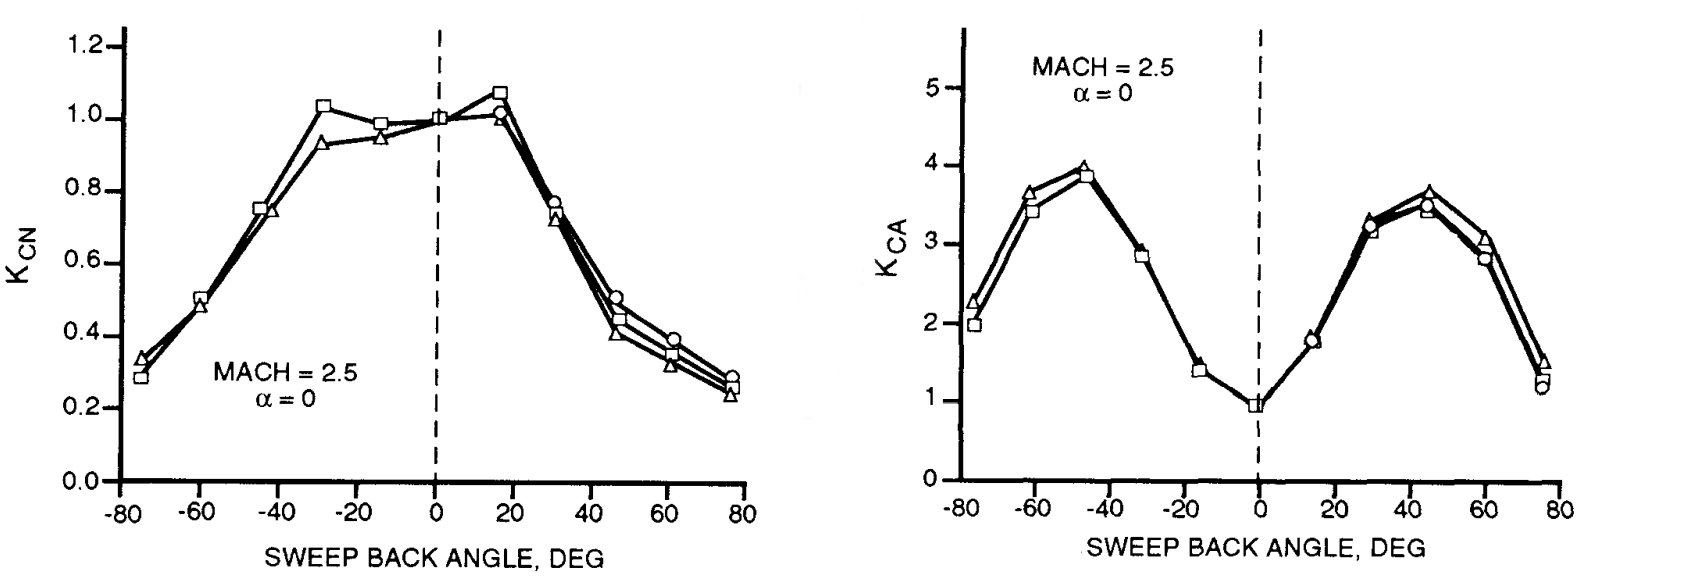
\includegraphics[width=0.95\textwidth]{PfeilKonf.png}
	\flushbottom{\cite{LambdaKonf}}
	\caption{Vielfache des Normalkraftanstiegs (links) und der Axialkraft (rechts) im Vergleich zum ungepfeilten Grid Fin in Abhängigkeit vom konfigurellen Pfeilungswinkel $\Lambda_{Konf}$ bei $Ma = 2,5$ und $\alpha = 0$}
	\label{abb_lastvielfache}
\end{figure}\\
Die zweite Variante ist eine \textbf{Pfeilung des Gitters} entlang der Steuerachse, sodass die auf die Y-Z-Ebene projizierte Geometrie unverändert bleibt. Das Ziel hierbei ist es die Axialkraft zu senken, indem die Verdichtungsstöße an den Gittervorderkanten nicht alle auf derselben Höhe liegen, sondern in X-Richtung gestaffelt stattfinden, sodass die Schockwelle nicht senkrecht, sondern schräg auf der luv-Seite ist. Abbildung \ref{abb_PfeilG} zeigt, wie ein ungepfeilter Grid Fin (links) zu einem gepfeilten (rechts) wird.
\begin{figure}[h]
	\centering
	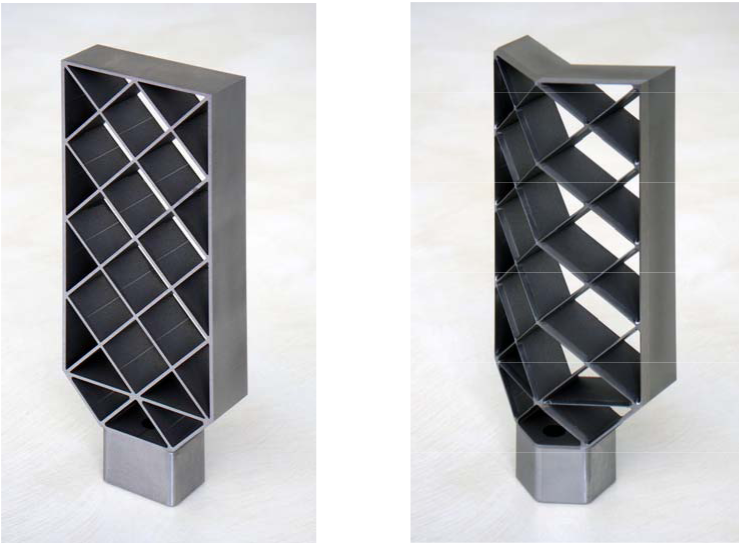
\includegraphics[width=0.6\textwidth]{PfeilGBild.png}
	\flushbottom{\cite{PfeilG3}}
	\caption{Ebener Grid Fin (links) und Grid Fin mit gepfeiltem Gitter (rechts)}
	\label{abb_PfeilG}
\end{figure}\\
In Abbildung \ref{abb_PfeilG-Ma} ist der Koeffizient der Axialkraft (links) und Anstieg des Normalkraftbeiwerts (rechts) für verschiedene Pfeilunswinkel $\Lambda_{G}$ über die Machzahl aufgetragen. Mit steigender Pfeilung des Gitters $\Lambda_G$ wächst die effektive Länge der Zellen, die als Düse fungieren. Der Stoß befindet sich somit näher an der Vorderkante und besitzt einen geringeren Winkel. Somit wird die Drosselung reduziert und die Expansionswellen am Zellausgang nehmen ab \cite{PfeilG1}. Dies sorgt dafür, dass im Bereich der kritischen Machzahlen die Axialkraft deutlich verringert wird. Auch der Gradient der Normalkraft $F_{N\alpha}$ nimmt mit steigenden Pfeilungswinkel im transsonischen Bereich zu \cite{PfeilG1}, was die Stabilität deutlich erhöht. Eine Vorwärtspfeilung $\Lambda_{G} < 0$ zeigt grundsätzlich ähnliche, wenn auch schwächere, Effekt wie die Rückwärtspfeilung \cite{PfeilG2}. Im Überschall lässt der Effekt auf die Axialkraft nach, sodass dieser vernachlässigbar wird. Für die Normalkraftgenerierung dreht sich die Wirkung der Pfeilung bei diesen Machzahlen sogar um, sodass schon bei $Ma_\infty=2$ der ungepfeilte Grid Fin dem gepfeilten überlegen ist.

Eine Pfeilung des Gitters birgt also hauptsächlich für den Transschall Vorteile wie geringere Axialkraft und einen erhöhten Normalkraftanstieg. Bei höheren Machzahlen bewirkt die Pfeilung jedoch auch bei letzterem eine Senkung, wodurch die Stabilität im Überschall reduziert wird.
\begin{figure}[h]
	\centering
	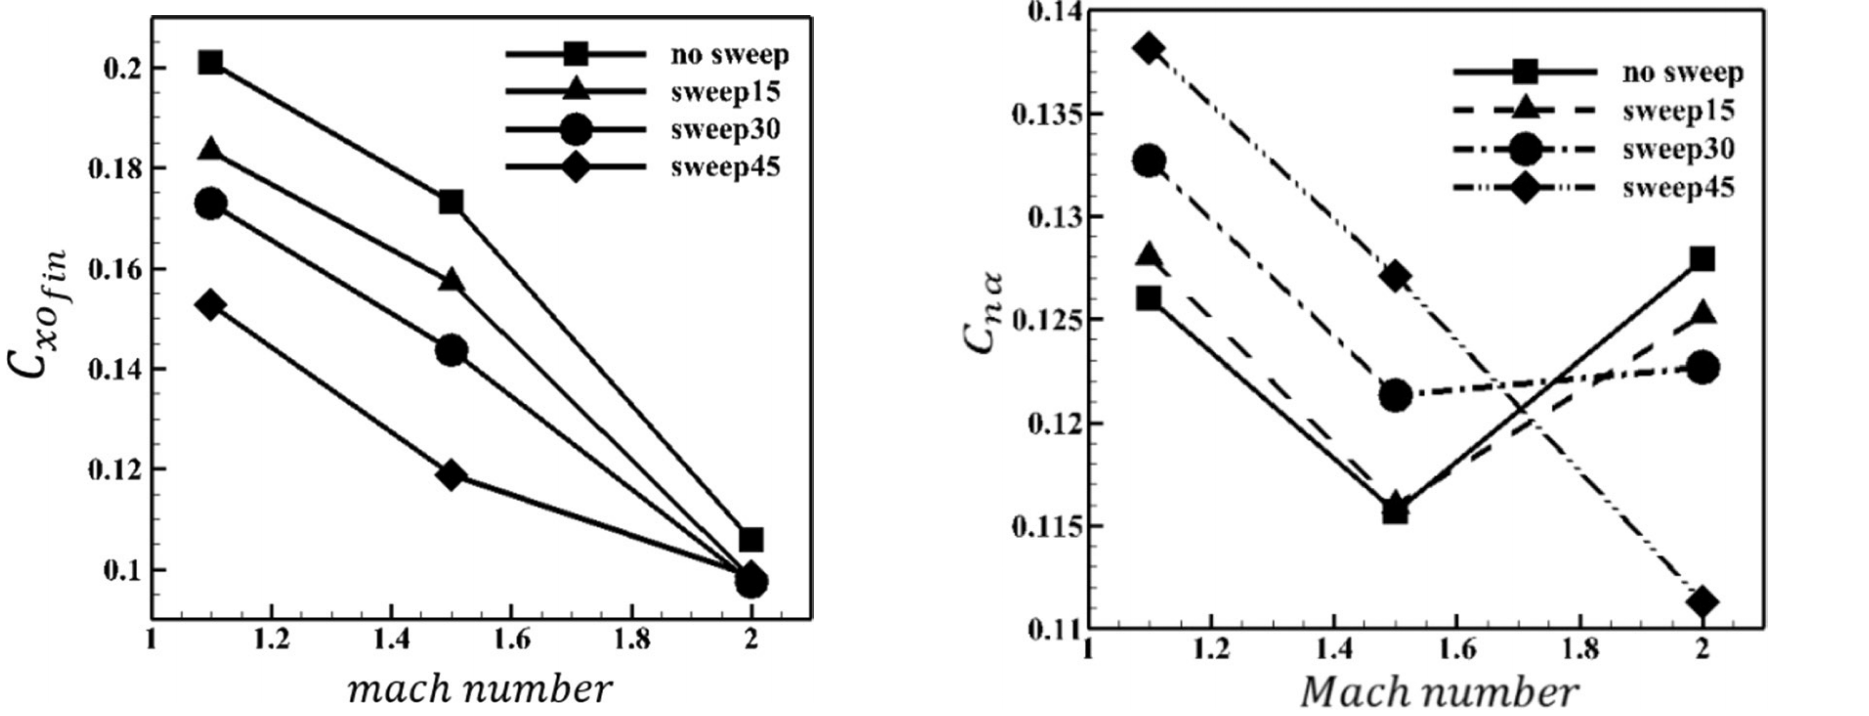
\includegraphics[width=0.95\textwidth]{PfeilG_Ma.png}
	\flushbottom{\cite{PfeilG1}}
	\caption{Axialkraftbeiwert (links) und Normalkraftsbeiwertanstieg (rechts) in Abhängigkeit von der Machzahl bei unterschiedlichen Pfeilungswinkeln $\Lambda_{G}$ und $\alpha = 0$}
	\label{abb_PfeilG-Ma}
\end{figure}\\
Als letzte Variante bleibt die \textbf{lokale Pfeilung der Zellwände} übrig. Diese kann man sich hierbei wie nebeneinander gereihte Deltaflügel vorstellen, sodass die luv-Seite des Grid Fins mit Zacken übersät ist. Für die Beschreibung dieser Pfeilung wird nicht nur der Winkel $\Lambda_{\gls{Index:Z}}$, sondern auch die Anzahl der Zähne pro Zelle und ihre Position relativ zu den Schnittstellen des Gitters, benötigt. Im Folgenden wird nur der Fall von einem Zahn zwischen zwei Schnittstellen der Zellwände betrachtet und die Eigenschaften beziehen sich auf ein Gitter, deren Vorder- und Hinterkanten nicht wie bisher betrachtet stumpf, sondern zugespitzt, sind. Auf unterschiedliche Kantenformen wird später in diesem Kapitel noch eingegangen. Für die Position der Spitze werden zwei Typen unterschieden, die in Abbildung \ref{abb_BergTal}. Beim Tal-Typus (b) befindet sich die Spitze in der Mitte der Zellwand, sodass sich an der Schnittstelle alle sich kreuzende Zellwände ein "Tal"\ teilen. Der Berg-Typus (a) hingegen hat ein Tal in der Mitte und benachbarte Zellen teilen sich einen "Berg".
\begin{figure}[h]
	\centering
	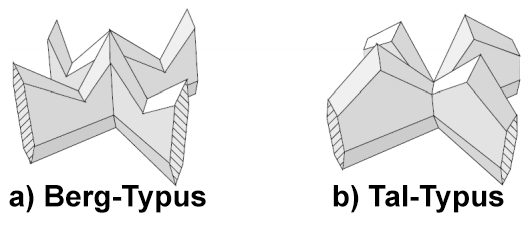
\includegraphics[width=0.6\textwidth]{PeakValley.png}
	\flushbottom{\cite{PeakValley}}
	\caption{Lokale Pfeilung der Zelle mit dem a) \grqq Berg\grqq -Typus und b) \grqq Tal\grqq -Typus}
	\label{abb_BergTal}
\end{figure}\\
Trifft nun eine Strömung auf lokal gepfeilte Gitterwände, so bilden sich an der Vorderkante drei verschiedene Druckbereiche. An der Spitze und von dort aus im Machkegel strömungsabwärts befindet sich eine 2D-Strömung, in deren Gebiet ein geringerer Druck an der Oberfläche herrscht. Im Tal hingegen kommt es zu deutlich erhöhtem Druck, da die Schockwellen der Pfeilung folgen und sich somit die der benachbarten Zähne hier kreuzen. Während die Größe dieser beiden Zonen relativ unabhängig von der Zahngröße ist, wachsen und schrinken die Ausmaße des Bereiches mit abgeschwächter Wellenintensität zwischen ihnen mit ihr \cite{PeakValley}.

Wird nun zuerst eine einzelne planare Wand unendlicher Streckung mit lokaler Pfeilung betrachtet, so zeigt sich eine Abnahme der Axialkraft mit steigenden Pfeilungswinkel $\Lambda_Z$ \cite{PeakValley}. Je hoher die Machzahl, dicker die Wandstärke und stumpfer die Vorderkante ist, desto stärker macht sich der Effekt bemerkbar. Im Gegensatz dazu verringert die Zahnlänge und der Anstellwinkel die Effektivität der lokalen Pfeilung \cite{PeakValley}.

Abbildung \ref{abb_PeakValley-Ma} zeigt den Koeffizienten des Wellenwiderstandes (links) und das Verhältnis von Auftrieb zum Widerstand (rechts) für lokal gepfeilte Gitter im Vergleich zu einem ungepfeilten.
Auch hier reduzieren beide Typen von lokaler Pfeilung den Wellenwiderstand deutlich. Beim Tal-Typus treffen jedoch vier statt nur zwei Wellen aufeinander, sodass es zu größeren Verlusten kommt und die Widerstandsreduzierung beim Berg-Typus bei einer Machzahl von $Ma=6$ um $1,2\%$ stärker ist \cite{PeakValley}.
Wie in Abbildung \ref{abb_PeakValley-Ma} zu sehen haben lokal gepfeilte Grid Fins auch ein höheres Auftrieb zu Widerstand Verhältnis, jedoch ist ihr Vorteil hier geringer, als beim Widerstand sodass ein geringerer Auftrieb vorzuliegen scheint. Zusätzlich zeigt an dieser Stelle der Tal-Typus bessere Eigenschaften, da seine Auftriebserzeugung über der des Berg-Typus liegt. 
\begin{figure}[h]
	\centering
	\includegraphics[width=0.9\textwidth]{PeakValley_Cd-Ma.png}
	\flushbottom{\cite{PeakValley}}
	\caption{Wellenwiderstandsbeiwert (links) und Auftrieb/Widerstand-Verhältnis (rechts) in Abhängigkeit von der Machzahl}
	\label{abb_PeakValley-Ma}
\end{figure}\\
Bei hohen Machzahlen lässt sich nun also mittels der lokalen Pfeilung der Zellwände, die Axialkraft auf Grid Fins stark vermindern. Dabei müssen jedoch leichte Einbußen in Bezug auf die Normalkraft in Kauf genommen werden.
\subsection{Krümmung}
Um das Transportpotenzial von Grid Fins am besten nutzen zu können, ist es wünschenswert, dass sie sich im eingeklappten Zustand an den Körper anschmiegen. Somit hätten sie, je nachdem ob sie in Flugrichtung ($\Lambda = -90^\circ$) oder entgegen ($\Lambda = 90^\circ$) gedreht werden, eine konkave oder konvexe Krümmung zur Anströmung, deren Radius dem vom Körper entspricht.

Dies hat unabhängig der Ausrichtung der Krümmung nur einen geringen Einfluss auf die Aerodynamik. Weder Axial- noch Normalkraft zeigen signifikante Änderungen \cite{LambdaKonf}, sodass die Leistungsfähigkeit erhalten bleibt. Beim Gelenkmoment zeichnen sich jedoch Unterschiede ab. Die konvexe Krümmung führt zu einem sehr kleinen Moment, dass sich für Anstellwinkel zwischen $\alpha = -10^\circ$ und $\alpha=20^\circ$ um die null bewegt \cite{LambdaKonf}. Für den konkaven Grid Fin zeigt sich jedoch ein Anstieg des Gelenkmomentes mit dem Anstellwinkel, der steiler ist als der des flachen \cite{LambdaKonf}. Hier sei jedoch anzumerken, dass sich die Werte noch immer in einem sehr niedrigen Bereich, deutlich unter planaren Finnen, bewegen.

Somit lässt sich mit einer Krümmung des Grid Fins, die der des Flugkörpers entspricht, die Transportmöglichkeiten ideal nutzen, ohne spürbare Einbußen in der Leistung zu haben.
\subsection{Wandquerschnitt}
Eine weitere Möglichkeit Grid Fins zu verändern ist die Variation des Wandquerschnitts und -dicke. Die Idee dahinter ist, dass die Strömung bisher schlagartig um eine stumpfe Vorderkante herum expandieren muss und somit große Axialkräfte bewirkt. Alternativ sind verschiedene Formen, wie zum Beispiel in Abbildung \ref{abb_Shape_Cd} (F2 bis F4) zu sehen, die das Fluid um eine Spitze Kante herum lenken.

Aus dieser Grafik lässt sich auch direkt die Reduktion an Axialkraft für alle dargestellten Machzahlen, durch eine Auftragung des Widerstandbeiwerts in Abhängigkeit von der Machzahl bei einem Anstellwinkel von $\alpha=0$, erkennen. Des Weiteren wird gezeigt, dass eine höhere Wanddicke des Gitters $d_G$ (F5) den Widerstand weiter steigert, was auch im Kontext einer stärkeren Verdrängung der Strömung Sinn ergibt. Ebenso führt ein dünnerer Rahmen $d_R$ (F6) zu einer Minderung der Kraft. Diese Trends scheinen unabhängig von der Machzahl zu sein. Weiter Untersuchungen von Miller und Washington haben ergeben, dass diese Unterschiede auch bei Variation des Anstellwinkels erhalten bleiben \cite{Shape}.

Die Normalkraft wird bei einer Machzahl von $Ma_\infty=0,7$ durch die Querschnittsform des Rahmens leicht beeinflusst. Über den gesamten Anstellwinkelbereich gibt es eine Variation von circa 10\% aufgrund der Form \cite{Pattern}. Ein dickeres Gitter führt in Unterschall jedoch zusätzlich zu einer leichten Abnahme der Normalkraft für Anstellwinkel $\alpha>10^\circ$ \cite{Pattern}. Bei kritischen Machzahlen und einem Anstellwinkel von $\alpha=5^\circ$ erreicht die Reduktion mit $13\%$ ein Maximum \cite{Pattern}. Im Überschall hingegen zeigt die erhöhte Wandstärke $d_G$ sogar eine leicht gesteigerte Normalkraft und der Effekt der Form hingegen ist vernachlässigbar gering.

Der Druckpunkt lässt sich durch eine veränderte Querschnittsform für die Beispiele F3 und F4 um ungefähr $5\%$ der Sehnenlänge $s$ nach hinten verschieben. Die führt im Unterschall, wo der Druckpunkt noch in der Nähe der $l/4$-Linie liegt, zu einer bemerkbaren Reduktion des Gelenkmomentes $M_m$ und im Überschall, wo der Druckpunkt ohnehin schon bei $45\%-50\%$ der Sehnenlänge liegt, zu Momenten, die für Anstellwinkel bis $\alpha<10^\circ$ fast gleich null sind \cite{Pattern}.

Mit einer gezielten Wahl des Querschnitts der Wände und Anpassung ihrer Dicke lässt sich die Axialkraft eines Grid Fins manipulieren, ohne Einbußen für Normalkraft und Gelenkmoment in Kauf nehmen zu müssen. Hierfür können sich unter bestimmten Bedingungen sogar auch positive Entwicklungen bemerkbar machen.
\begin{figure}[h]
	\centering
	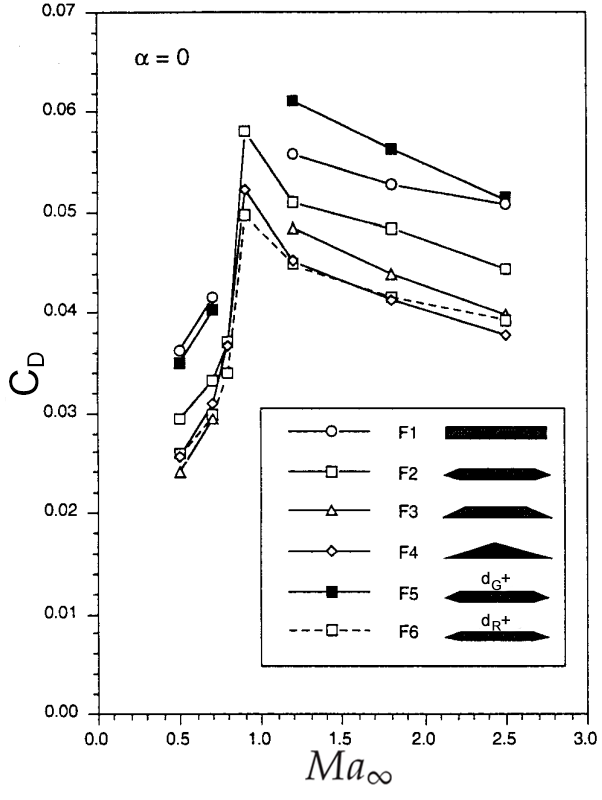
\includegraphics[width=0.4\textwidth]{Shape_Cd-Ma.png}
	\flushbottom{\cite{Shape}}
	\caption{Widerstandsbeiwert für verschiedene Rahmenquerschnittsformen (F1-F4), einen dickeren Rahmen $d_R$ (F5) und ein dünneres Gitter $d_G$ (F6) bei $\alpha = 0$ in Abhängigkeit von der Machzahl}
	\label{abb_Shape_Cd}
\end{figure}

\subsection{Zellform}
Für die Form der einzelnen Zellen sind unterschiedliche Varianten denkbar. Neben Rechtecken sind auch Dreiecke möglich, welche der Struktur eine noch höhere Stabilität verleihen. Alternativ wäre für den idealen Durchlass der Strömung eine runde Zelle am besten, um die Axialkraft zu minimieren. Da mit Kreisen keine Fläche lückenlos füllbar ist, kann hier auf eine bienenwabenähnliche Sechseckstruktur also gut Näherung zurückgegriffen werden \cite{Pattern}. In Abbildung \ref{abb_parameter} ist auch schon eine Kombination unterschiedlich geformter Zellen zu sehen, was eine flexible Gestaltung der Gesamtgitterform ermöglicht.\\
Abbildung \ref{abb_Form-Cn} zeigt den Anstieg des Normalkraftkoeffizienten in Abhängigkeit von der Machzahl für quadratische, dreieckige und sechseckige Zellen mit gleicher Querschnittsfläche pro Zelle und Zellanzahl.
Weder im Unter- noch im Überschall zeigen die unterschiedlichen Zellformen bei gleicher Gesamtquerschnittsfläche $A$ einen signifikanten Unterschied in Bezug auf die Normalkraft und das Gelenkmoment \cite{Pattern}. Die Auftriebsfläche, der Anteil der Zellwände die orthogonal zur Y-Achse liegen, scheint somit keinen großen Einfluss auf den Auftrieb zu haben, da sie bei den Sechsecken deutlich geringer ist. Nur im Transschall machen sich wieder besondere Effekte bemerkbar. Der Normalkraftsbeiwertanstieg der Wabenstruktur ist in der Ausgangsstellung $\alpha = 0$ deutlich unter den Werten des Drei- und Viereckgitters \cite{Pattern}. Die Normalkraft steigt im Gegensatz zu dem nicht-linearen Verhalten der beiden anderen Zellformen bei den Sechsecken jedoch konstant an, sodass bei hohen Anstellwinkeln wieder kein wirklicher Unterschied bemerkbar ist \cite{Pattern}.\\
Die Zellform hat folglich nur einen geringen Einfluss auf die aerodynamischen Eigenschaften eines Grid Fins.
\begin{figure}[h]
	\centering
	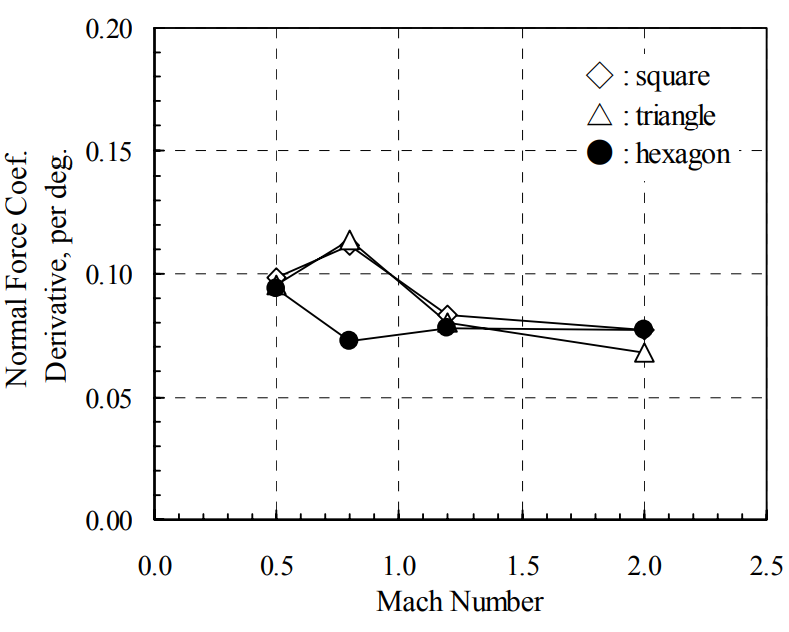
\includegraphics[width=0.5\textwidth]{Pattern_CNa.png}
	\flushbottom{\cite{Pattern}}
	\caption{Anstieg des Normalkraftkoeffizienten über den Anstellwinkel $\alpha$ in Abhängigkeit von der Machzahl für verschiedene Zellformen bei $\alpha = 0$}
	\label{abb_Form-Cn}
\end{figure}
\subsection{Zellgröße}
Während die Größe der Querschnittsfläche $A$ als Referenzfläche die Kräfte proportional mit sich verändert, ist der Einfluss der Zellgröße $g$ ist weniger offensichtlich. Klar sind die Extreme. Entspricht die Zellgröße der Dimension des gesamten Grid Fins, besteht dieser nur aus einem Rahmen. Somit kann es nur eine minimale Axialkraft geben und auch für die Normalkraft fehlt so gut wie jegliche Wirkfläche. Geht im Gegensatz dazu die Zellgröße $g$ gegen null. Wirkt der Grid Fin wie eine planare Ebene senkrecht zur Strömung, die eine sehr große Axialkraft induziert. Auch die Normalkraft ist hier sehr gering, da die Strömung wie bei planaren Finnen unter hohen Anstellwinkeln abreißt. Es ist nun also ein angemessenes Mittelmaß zu finden, dessen Normalkraft, unter Berücksichtigung eines annehmbaren Wiederstandes, ein Maximum einnimmt.

Tripathi et al. haben eine rudimentäre Grid Fin Konstruktion, die Kaskaden Finne, betrachtet. Diese besteht aus mehreren übereinander gestapelten planaren Flächen, die außen mit einer Wand verbunden sind, sodass sich auch hier Zellen bilden. Sie haben das Verhältnis zwischen Sehnenlänge und Abstand der planaren Flächen, was der Zellgröße entspricht, variiert \cite{ChordVar}, um den Effekt auf die Aerodynamik zu untersuchen.

In Abbildung \ref{abb_Gap-Chord} ist der Anstieg des Normalkraftbeiwerts in Abhängigkeit von diesem Verhältnis dargestellt. Für den Unterschall lässt sich somit ein klares Maximum erkennen, welches in diesem Beispiel eintritt, wenn Sehne und Zellabstand den selben Wert annehmen $g=s$.
Die Axialkraft hingegen nimmt mit einen Anstieg des Verhältnisses stetig zu \cite{ChordVar}, obwohl der Zellabstand konstant gehalten wird und nur die Sehnenlänge variiert. Da jedoch in den von Tripathi et al. durchgeführten Untersuchungen die Breite der planaren Ebenen an die Sehnenlänge gekoppelt ist, wird mit steigendem Zellabstand zu Sehnenlänge Verhältnis die durchströmte Querschittsfläche kleiner. Dies zeigt, dass dem zu Trotz eine kompaktere Struktur mehr Widerstand erzeugt \cite{ChordVar}. Der Anstieg des Widerstandes ist auch bei kleinen Verhältnissen größer als die Zunahme an Normalkraft für alle untersuchten Anstellwinkel, sodass das beste Auftrieb zu Widerstandsverhältnis bei den niedrigsten Zellgröße zu Sehnenlänge Verhältnissen auftritt \cite{ChordVar}.
\begin{figure}[h]
	\centering
	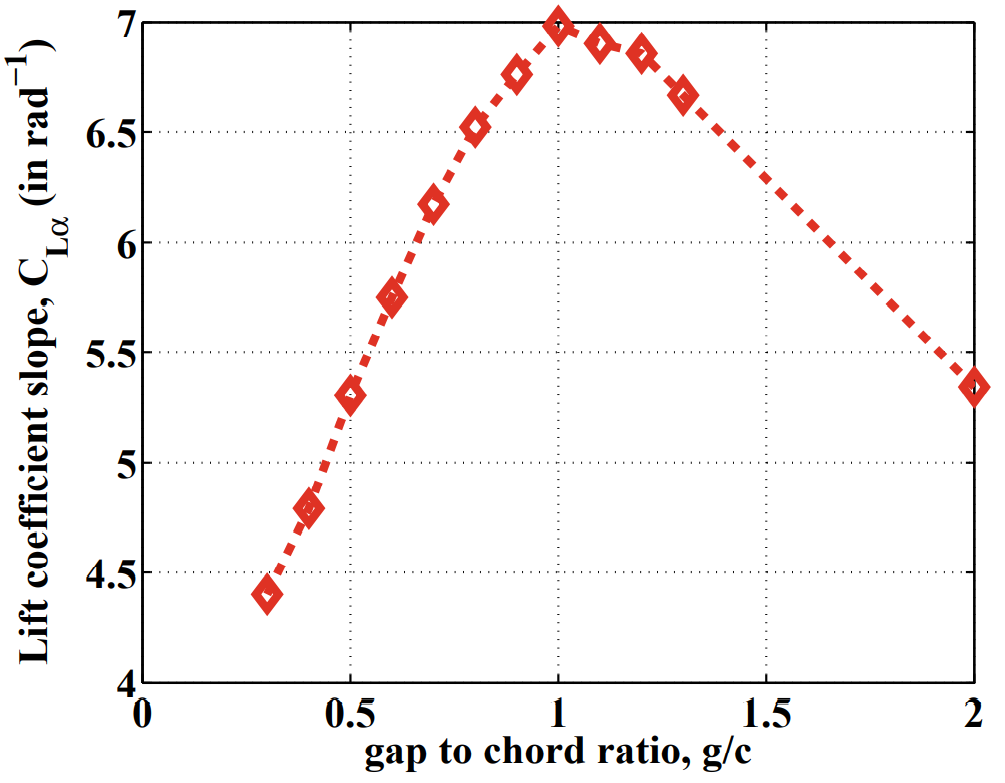
\includegraphics[width=0.5\textwidth]{Gap-to-Chord.png}
	\flushbottom{\cite{Pattern}}
	\caption{Anstieg des Normalkraftkoeffizienten in Abhängigkeit des Verhältnis zwischen Zellgröße und Sehnenlänge für Kaskaden Finnen bei $Ma_\infty = 0,1176$}
	\label{abb_Gap-Chord}
\end{figure}\\
Es gibt also einen Punkt für den Zellabstand, bei dem das Gitter den größten Normalkraftgradienten zeigt. Spielt bei der Auslegung die Axialkraft jedoch eine Rolle, kann es sein, dass von diesem Wert abgewichen werden muss.
\newpage
\section{Bisherige Implementierung}
Es wird nun ein Blick auf bisherige Anwendungen von Grid Fins geworfen. Da sie jedoch bisher hauptsächlich für ballistische Raketen verwendet wurden und sich die Anforderungen im Vergleich zur Raumfahrt um einiges unterscheiden können, werden hier nur Beispiele des letzteren betrachtet.
\subsection{SpaceX Falcon 9 und Starship}
SpaceX hat mit der ersten Stufe der Falcon 9 den wohl bekanntesten Vertreter von Grid Fins in der Raumfahrt. Diese werden genutzt, um beim Wiedereintritt den Booster aerodynamisch zu steuern. 

Abbildung \ref{abb_finsF9} zeigt zwei verschiedene Versionen dieser Grid Fins, das ältere Modell 3 (links) und das neuere Modell 4 (rechts). Beide haben insgesamt eine Rechteckige Struktur und bestehen aus einem Quadratgitter, das am Rahmen durch Dreiecke ergänzt ist. Die Querschnittsfläche der Wände hat eine einfache Rechteckform mit stumpfen kannten. Die Finnen lassen sich nach unten ($\Lambda = 90^\circ$) einklappen und haben eine konkave Krümmung. Ihre Einspannung scheint ähnlich aufgebaut zu sein, sodass sie sich um zwei Freiheitsgrade, den Klapp- und Steuerwinkel, bewegen können. Als Aktuator zur Steuerung um diese zwei Achsen werden hydraulische Pumpen verwendet. Zusätzlich haben beide Versionen an der der Anbringung gegenüberliegenden Seite einen Mechanismus, der sie in der eingeklappten Position zu halten scheint. Die Wanddicke $d$ der Grid Fins nimmt mit steigender Entfernung zur Anbringung ab. Bei der älteren Version, Mod 3 in Abbildung \ref{abb_finsF9} links zu sehen, ist der Unterschied der rechts zu erkennenden Mod 4, da jene noch zwei zusätzliche Stützstreben besitzt, die sich durch den gesamten Grid Fin ziehen. In dem neueren Modell wurden diese durch einzelne dünne Wände, die die oberen Zellen halbieren, ersetzt. Auch die Verstärkung für den Klappmechanismus konnte beim Mod 4 weggelassen werden. Allgemein weist die Oberfläche der Falcon 9 auf der rechten Seite von Abbildung \ref{abb_finsF9} weniger Erhebungen auf und besonders der Festhaltemechanismus nimmt eine neue Position ein, die zur Unregelmäßigkeit im Gitter führt. Beim genaueren Hingucken ist beim Mod 4 eine wellige Struktur auf der Unterseite, die beim Wiedereintritt zur Strömung zeigt. Diese ist eine abgerundete Variante der lokalen Pfeilung der Zellwände in Berg-Typus. Neben den Veränderungen der Geometrie wurde auch der verwendete Werkstoff mehrmals gewechselt. Während noch die ersten Modelle aus Aluminium bestanden und somit teilweise bei den extremen Missionsbedingungen schmolzen \cite{titanium}, wurden diese später durch hitzebeständigere Titanfinnen ausgetauscht, welche die Wiedereintrittstemperaturen ohne Hitzeschild aushalten, sodass sie laut Elon Musk ohne Aufbereitung eine unbegrenzt Anzahl von Missionen durchführen können (Quelle: Twitter @elonmusk).
\begin{figure}[h]
	\centering
	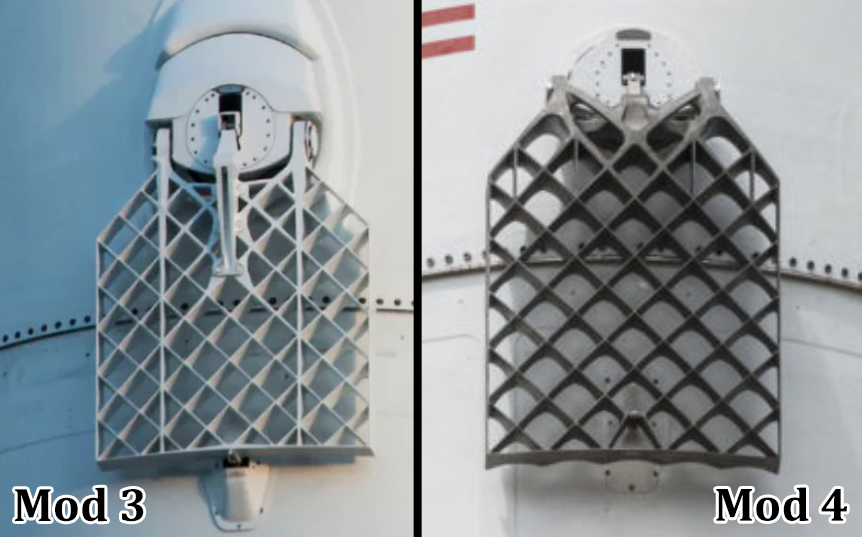
\includegraphics[width=0.75\textwidth]{fins-F9.png}
	\flushbottom{Quelle: SpaceX}
	\caption{Grid Fins an der Falcon 9, Version Mod 3 links und Mod 4 rechts}
	\label{abb_finsF9}
\end{figure}\\
Der Super Heavy Booster für SpaceX's Starship, wie in Abbildung \ref{abb_starship} zu sehen, soll auch Grid Fins erhalten. Da es noch keine Flüge dieser Erststufe gab (Stand: 21.05.2021), sind noch nicht viele Informationen über die Grid Fins bekannt. Auf ersten von SpaceX veröffentlichen Illustrationen lässt dich jedoch schon eine unsymetrische Sechseckform des Rahmens erkennen. Das Quadratgitter hat dadurch am Rand im Gegensatz zu den Finnen des Falcon 9 Boosters nur unregelmäßige Dreiecke an der Außenkante. Wie auch schon das Mod 4, sollen auch diese ein örtliche Pfeilung der Zellwände besitzen.

Die größte Änderung ist wohl die Materialwahl. Hierbei ist die Entscheidung weder auf Aluminium noch Titan gefallen, sondern auf den Edelstahl SS301 oder auch DIN 1.4310 genannt \cite{titanium}. Dieser rostfreie Stahl hat zwar eine Schmelztemperatur, die unter der von Titan liegt, jedoch sich die mechanischen Eigenschaften sehr ähnlich und werden sogar bis zu Temperaturen von bis zu $840^\circ C$ im Gegensatz zu den $330^\circ C$ von Titan aufrecht erhalten \cite{titanium}. Einer der größten Vorteile ist aber von wirtschaftlicher Natur, da Titan das 15- bis 20-fache von diesem Stahl kostet \cite{titanium}. Auch die Fertigung gestaltet sich mit dem günstigeren Werkstoff einfacher. Während die Grid Fins für die Falcon 9 in einem Stück gegossen und im Nachhinein noch durch trennende Verfahren bearbeitet werden (Quelle: Twitter @elonmusk), sollen beim Starship die deutlich größeren Grid Fins zusammen geschweißt werden.
\begin{figure}[h]
	\centering
	\includegraphics[width=\textwidth]{starship.png}
	\flushbottom{Quelle: SpaceX}
	\caption{SpaceX's Starship inklusive Super Heavy Booster}
	\label{abb_starship}
\end{figure}\\
\subsection{Sovietische Sojus und N-1}
Da Grid Fins in der Soviet Union erstmals entwickelt wurden, ist es kein Wunder, dass sie auch hier Anwendung in der Raumfahrt gefunden haben. So zeigt zum Beispiel Abbildung \ref{abb_sojus} das Notfall-Rettungssystem, mit dem sich die Astronauten an Bord bei Komplikationen von der Sojus Rakete trennen können. Diese Grid Fins beschränken sich hier hauptsächlich auf eine Funktion als drag brakes \cite{soyuz}. Ihre Rahmen haben eine Quadratische Form, wie auch die Zellen. Analog zu den Grid Fins der Falcon 9 befinden sich außen dreieckige Zellen und es existiert ein Mechanismus, der die Finnen im eingeklappten Zustand hält. Diese befindet sich jedoch hier oberhalb der Anbringung, da bei der sowjetischen Variante die Grid Fins nach oben geklappt sind.
\begin{figure}[h]
	\centering
	\includegraphics[width=0.3\textwidth]{sojus.png}
	\flushbottom{Quelle: NASA}
	\caption{Das Sojus Notfall-Rettungssystem mit Grid Fins}
	\label{abb_sojus}
\end{figure}\\
Auch die Sovietische Mondrakete Nositel 1 war mit vier Grid Fins ausgestattet, die sich denen der Sojus sehr ähneln, sodass auf sie hier nicht weiter eingegangen wird.

\subsection{Chinas Chang'e}
Auch in Chinas Raumfahrtbrache habe Grid Fins ihren Einzug erfahren. Das Bild in Abbildung \ref{abb_change} von 2019 zeigt, dass hier die Steuerflächen denen der Falcon 9 wieder deutlich ähnlicher sehen. Neben den offensichtlichen Gemeinsamkeiten, sind jedoch die komplexeren Strukturen weggelassen worden. So gibt es zum Beispiel weder Krümmung noch Pfeilung. Des Weiteren scheint die Sehne nahezu doppelt so lange wie die Zellgröße zu sein, im Gegensatz zur Falcon 9 mit einem Verhältnis von circa $1:1$.
\begin{figure}[h]
	\centering
	\includegraphics[width=\textwidth]{chang'e.png}
	\flushbottom{Quelle: China Aerospace Science and Technology Corporation}
	\caption{Die Grid Fins der chinesischen Chang'e}
	\label{abb_change}
\end{figure}\\
\newpage
\section{Das Air-Launchsystem Valkyrie}
Um die Anforderungen an eine Grid Fin Aktuatorik definieren zu können, ist eine vorherige Betrachtung der Mission von Nöten, diese, wie in Abbildung \ref{abb_valkMission} dargestellt, wird in diesem Abschnitt erläutert. Wie schon in der Einleitung erwähnt, handelt es sich bei der Valkyrie um ein wiederverwendbares, zweistufiges AirLaunch-System.  Relevant ist für diese Arbeit nur die Erste Stufe, an der die Grid Fins montiert sind.

Die Rakete wird an einem Flugzeug befestigt auf eine typische Reisehöhe von $11$km gebracht \cite{flugbahnBarz}. Dort wird sie von den Pylonen gelöst und nach $3$s zünden die Triebwerke der ersten Stufe. Nach eine Brenndauer von $170$s\textbf{???} werden diese wieder abgeschaltet und $5$s später kommt es zur Separation der beiden Stufen \cite{flugbahnBarz}. Während kurze Zeit später die zweite Stufe ihre Triebwerke zündet, um die Nutzlast in den Orbit zu befördern, bewegt sich die erste Stufe ohne weiteren Antrieb auf ihrer Suborbitalen Bahn fort. Dabei benutzt sie ihr Reaction Control System (RCS), um die Raketenstufe so zu drehen, dass beim Wiedereintritt die Triebwerke der Anströmung entgegen zeigen. Somit kann ein ungefähr $27$s\textbf{???} langer ReEntry-Burn durchgeführt werden, der die Fluggeschwindigkeit weit genug abbremst, um die Belastungen beim Wiedereintritt zu reduzieren. Des Weiteren sollen die Triebwerke in der Atmosphäre die Raketenstufe dank ihrer hohen thermischen Belastbarkeit durch aerodynamischen Widerstand weiter abbremsen. Noch vor dem ReEntry-Burn sollen die Grid Fins ausgefahren werden. Diese sorgen während des Fluges durch die Atmosphäre für Stabilität und Steuerbarkeit. Bei einer Höhe von unter $20$km und einer Geschwindigkeit $Ma<2$ wird der Ballonschirm eingesetzt \cite{flugbahnBarz}. Dieser bremst die Rakete weiter bis in den Unterschall ab, sodass ein Fallschirm geöffnet werden kann. Der wiederum eine Bergung mittels Helikopter und Skyhook ermöglicht.
\begin{figure}[h]
	\centering
	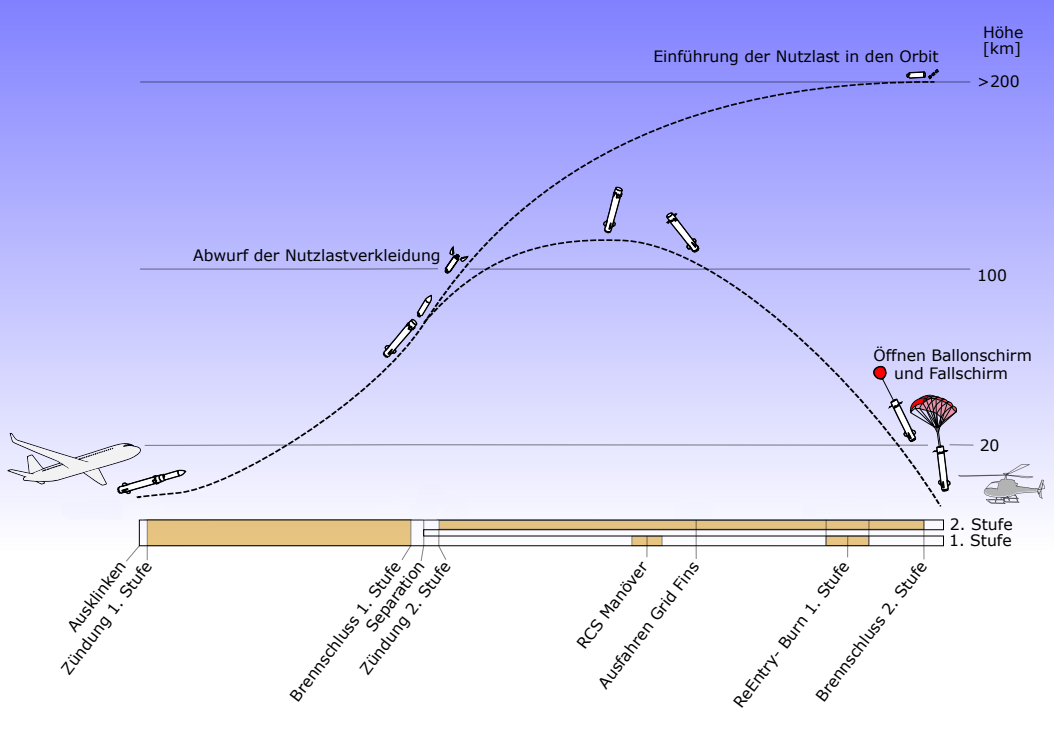
\includegraphics[width=0.8\textwidth]{ablauf_valkyrie_zeitlos.png}
	\flushbottom{\cite{flugbahnBarz}}
	\caption{Der Ablauf einer Valkyrie Mission}
	\label{abb_valkMission}
\end{figure}\\

